\begin{tikzpicture}[scale=1]
    \node at (0.2,1) {$t$};
    \node at (0,0.3) {
\includegraphics[width=5mm]{runner.jpg}};
    \node at (2.5,0.35) {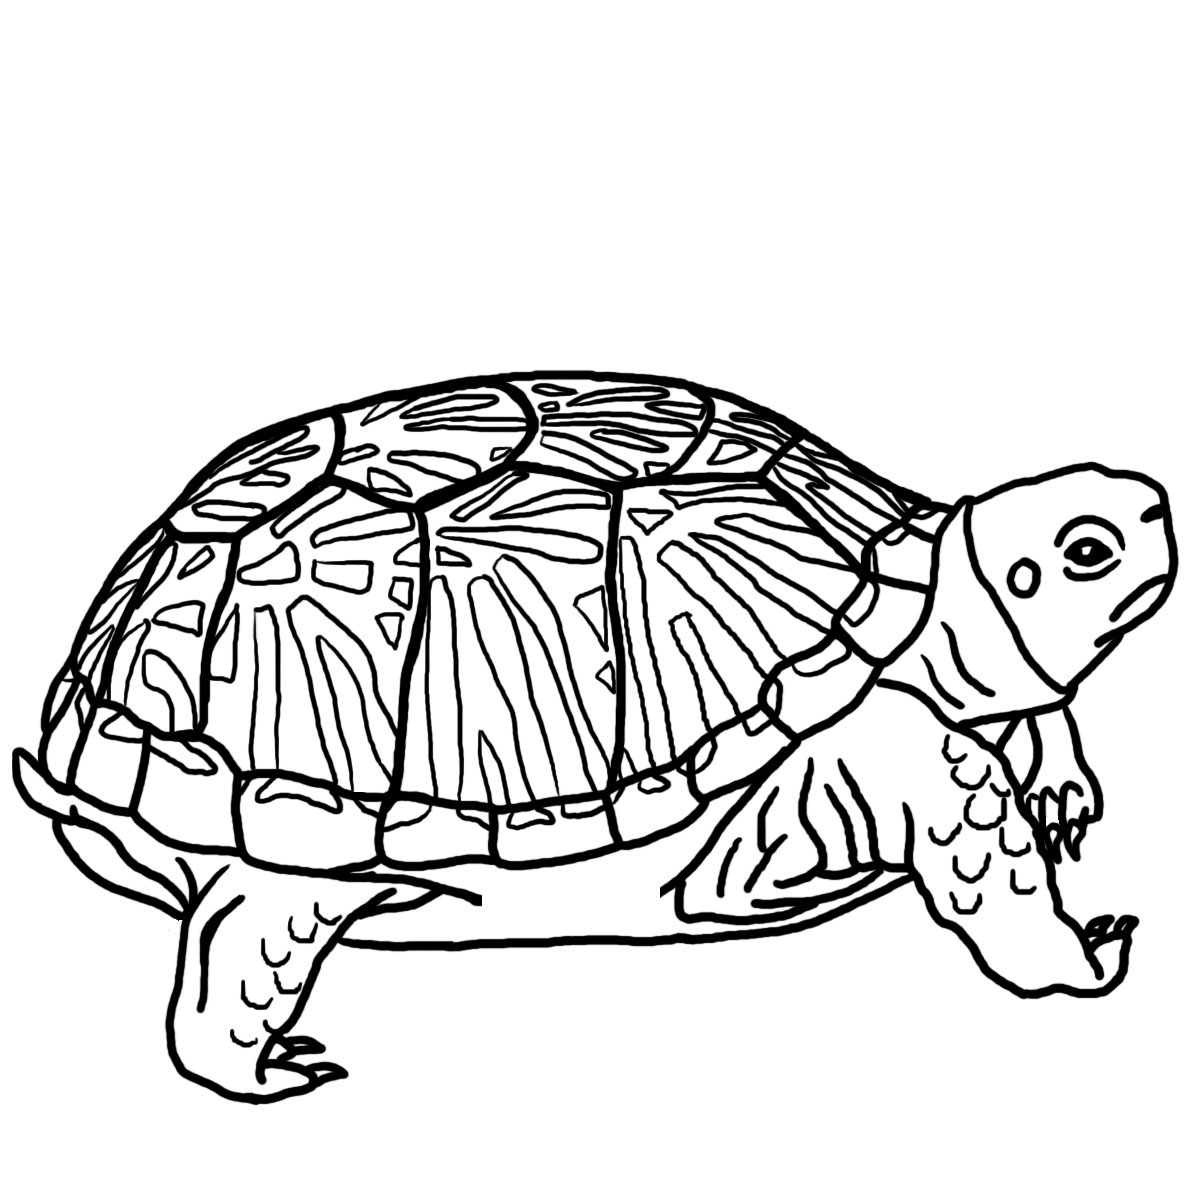
\includegraphics[width=8mm]{turtle.jpg}};
    \draw[->] (0,0) -- (5,0);
    \draw[] (0,-0.2) node[below] {0} -- (0,0.1);
    \draw[] (2.5,-0.2) node[below] {\SI{100}{\metre}} -- (2.5,0.1);
    %t=1s
    
    \begin{scope}[shift={(0,-2)}]
        \node at (0.2,1) {$2t$};
        \node at (2.5,0.3) {
\includegraphics[width=5mm]{runner.jpg}};
        \node at (3.75,0.35) {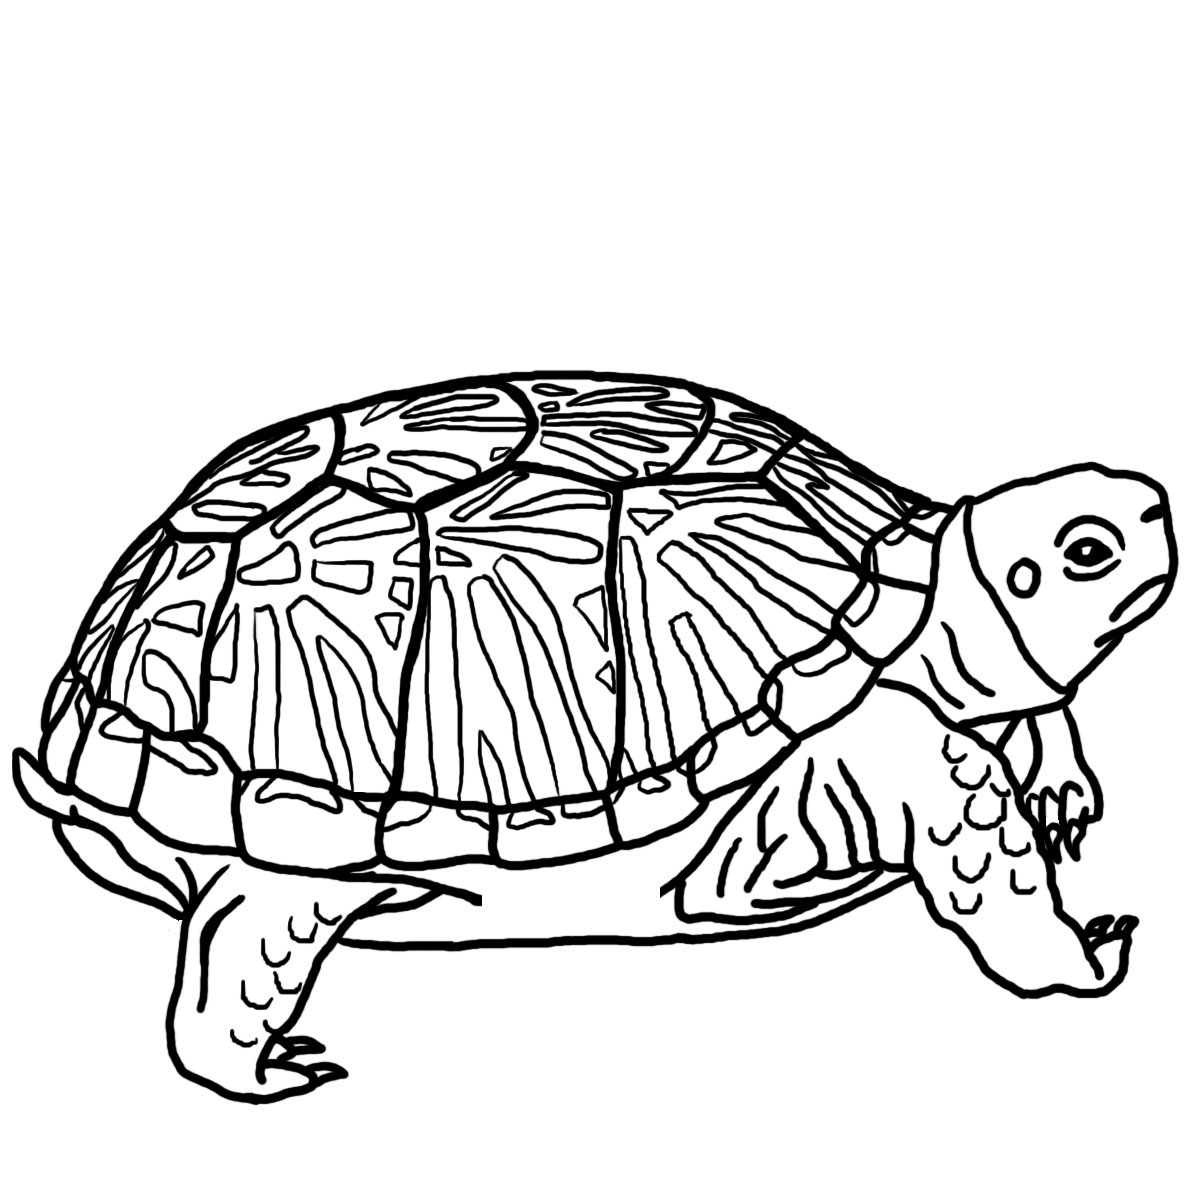
\includegraphics[width=8mm]{turtle.jpg}};
        \draw[->] (0,0) -- (5,0);
        \draw[] (0,-0.2) node[below] {0} -- (0,0.1);
        \draw[] (2.5,-0.2) node[below] {\SI{100}{\metre}} -- (2.5,0.1);
        \draw[] (3.75,-0.2) node[below] {\SI{150}{\metre}} -- (3.75,0.1);
    \end{scope}

    
\end{tikzpicture}